\subsubsection{Top Level}
At the top level, design parameters are passed from the user to the pod, tube, mission, and ticket cost subsystems which then all output variables to the user.
	\begin{figure}
		\centering
		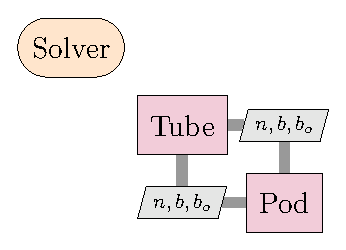
\includegraphics{../images/xdsm/tube_and_pod.pdf}
		\caption{XDSM diagram for entire system model}
		\label{fig:xdsm:toplevel}
	\end{figure}
\subsubsection{Pod}
	\begin{figure}
		\centering
		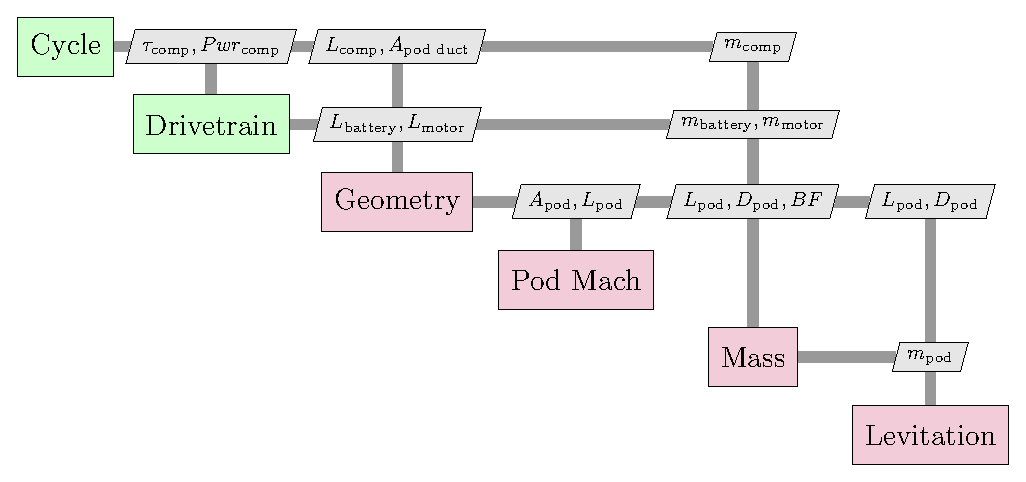
\includegraphics{../images/xdsm/pod.pdf}
		\caption{XDSM diagram for Pod group}
		\label{fig:xdsm:pod}
	\end{figure}
\subsubsection{Tube}
	\begin{figure}
		\centering
		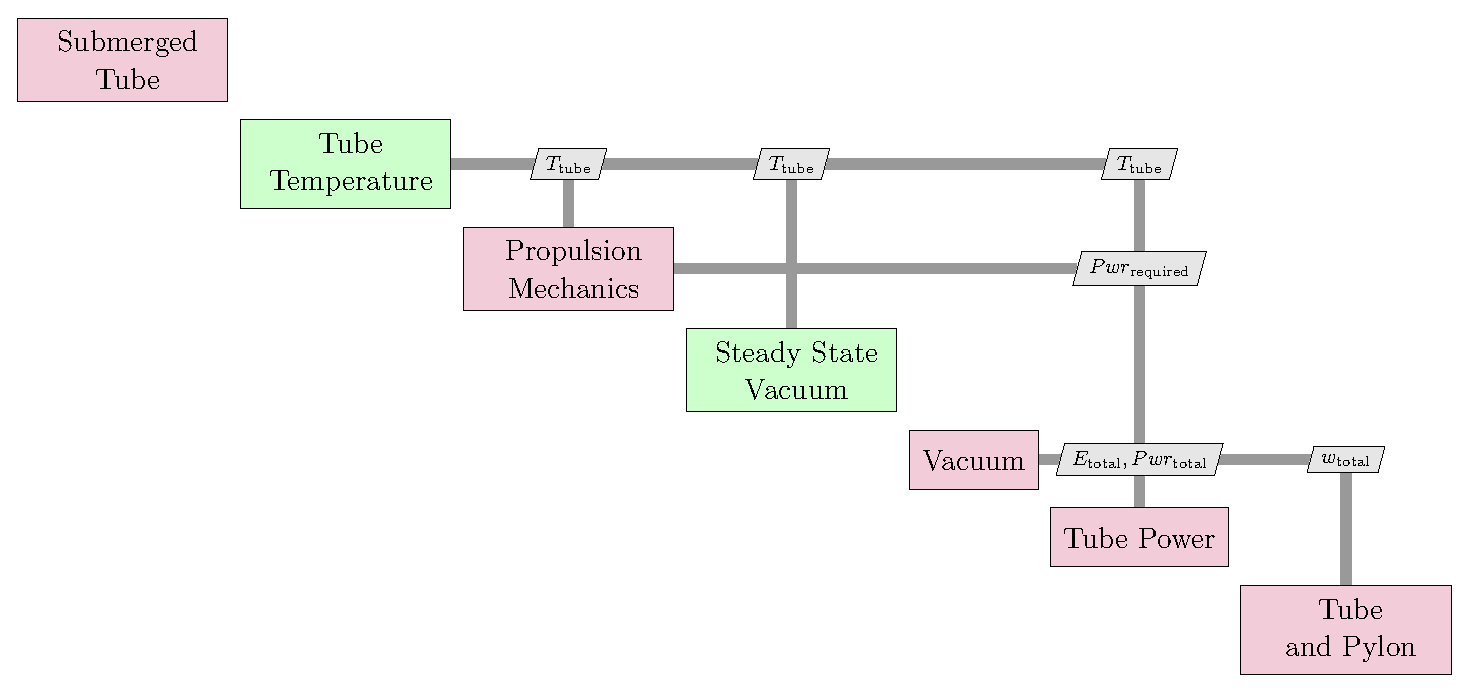
\includegraphics{../images/xdsm/tube.pdf}
		\caption{XDSM diagram for Tube group}
		\label{fig:xdsm:tube}
	\end{figure}
	